\chapter{Аналитический раздел}

В данном разделе будет представлены основные сведения о способах хранения разреженных матриц. Также будет описано условие задачи и техническое задание.

\section{Способы хранения разреженных матриц}

Существуют различные методы хранения элементов матрицы в памяти. Например, линейный связный список, т.е. последовательность ячеек, связанных 
в определенном порядке. Каждая ячейка списка содержит элемент списка и указатель 
на  положение  следующей  ячейки.  Можно  хранить  матрицу,  используя  кольцевой 
связный список, двунаправленные стеки и очереди. Существует диагональная схема 
хранения  симметричных  матриц,  а  также  -  связные  схемы  разреженного  хранения. 
Связная схема хранения матриц, предложенная Кнутом, предлагает хранить в массиве 
(например, в AN) в произвольном порядке сами элементы, индексы строк и столбцов 
соответствующих  элементов  (например,  в  массивах  I  и  J),  номер  (из  массива  AN) 
следующего  ненулевого  элемента,  расположенного  в  матрице  по  строке  (NR)  и  по 
столбцу (NC), а также номера элементов, с которых начинается строка (указатели для 
входа в строку –  JR) и номера элементов, с которых начинается столбец (указатели 
для  входа  в  столбец  -  JC).  Данная  схема  хранения  избыточна,  но  позволяет  легко 
осуществлять любые операции с элементами матрицы.  

Наиболее  широко  используемая  схема  хранения  разреженных  матриц  -  это 
схема, предложенная Чангом и Густавсоном, называемая: "разреженный строчный 
формат". Эта схема предъявляет минимальные требования к памяти и очень удобна 
при  выполнении  операций  сложения,  умножения  матриц,  перестановок  строк  и 
столбцов, транспонирования, решения систем линейных уравнений, при хранении 
коэффициентов в разреженных матрицах и т.п. 
В  этом  случае  значения  ненулевых  элементов  хранятся  в  массиве  AN, 
соответствующие им столбцовые индексы -  в массиве JA. Кроме того, используется 
массив  указателей,  например, IA,  отмечающих  позиции  AN и  JA,  с  которых 
начинаются описание очередной строки. Дополнительная компонента в IA  содержит 
указатель первой свободной позиции в JA и AN.

В связи с тем, что разреженный строчный формат предъявляет минимальные требования к памяти и удобна для операции умножения, в данной лабораторной работе будет использована именно она.

\section{Описание условия задачи}

Разработать  программу  умножения  или  сложения  разреженных  матриц. 
Предусмотреть  возможность  ввода  данных,  как  с  клавиатуры,  так  и  использования 
заранее  подготовленных  данных.  Матрицы  хранятся  и  выводятся  в  форме  трех 
объектов.  Для  небольших  матриц  можно  дополнительно  вывести  матрицу  в  виде 
матрицы. Величина матриц -  любая (допустим, $1000\times1000$). Сравнить эффективность 
(по памяти и по времени выполнения) стандартных алгоритмов обработки матриц с 
алгоритмами обработки разреженных матриц при различной степени разреженности 
матриц и различной размерности матриц.

\section{Техническое задание}

Разреженная (содержащая много нулей) матрица хранится в форме 3-х объектов:
\begin{itemize}[$\bullet$]
	\item вектор A содержит значения ненулевых элементов; 
	\item вектор JA содержит номера столбцов для элементов вектора A; 
	\item связный список IA, в элементе Nk которого находится номер компонент 
	в A и JA, с которых начинается описание строки Nk матрицы A. 
\end{itemize}

\begin{enumerate}
	\item Смоделировать операцию умножения вектора-строки и матрицы, 
	хранящихся в этой форме, с получением результата в той же форме. 
	\item Произвести операцию умножения, применяя стандартный алгоритм работы с 
	матрицами. 
	\item Сравнить время выполнения операций и объем памяти при использовании 
	этих 2-х алгоритмов при различном проценте заполнения матриц. 
\end{enumerate}

\section{Вывод}

В данном разделе были описаны способы хранения матриц в памяти и сформулировано техническое задание. В результате анализа способов хранения матриц для реализации операции умножения вектора-строки на матрицу был выбран разреженный строчный формат хранения.


\chapter{Конструкторский раздел}

В данном разделе будут описаны используемые структуры данных, приведен список функций для работы с данными типами. Также будет описан алгоритм умножения разреженных матриц.


\section{Описание структур данных}

Ниже, на листинге \ref{errors} представлены коды возможных ошибок.

\begin{lstlisting}[label=errors,language=C,caption=Коды ошибок]
#define SUCCESS     0   // Успешное выполнение
#define MEM_ERR     1   // Ошибка памяти
#define INP_ERR     2   // Ошибка ввода
#define BAD_MATRIX  3   // Некорректная матрица
#define BAD_PERCENT 4   // Некорректный процент заполнения
#define ARGS_ERR    5   // Некорректные аргументы, переданные в функцию
#define MUL_ERR     6   // Матрицы невозможно перемножить
#define BAD_VECTOR  7   // Вектор некорректен
#define BAD_FILE    8   // Файл некорректен
\end{lstlisting}

Ниже, на листинге \ref{types} представлены сокращения используемых типов данных.

\begin{lstlisting}[label=types,language=C,caption=Используемые типы]
typedef double data_t;
typedef unsigned int id_t;
\end{lstlisting}

Ниже, на листинге \ref{lst} представлена структура связного списка.

\begin{lstlisting}[label=lst,language=C,caption=Связный список и функции для работы с ним]
typedef struct node
{
	id_t col_index;    // индекс столбца
	struct node* next; // следующий элемент
} node_t;

typedef struct list
{
	node_t* head;   // указатель на голову
} list_t;
\end{lstlisting}

На листинге \ref{smat}, представленном ниже, описана структура разреженной матрицы и функции для работы с ней.

\begin{lstlisting}[label=smat,language=C,caption=Разреженная матрица и функции для работы с ней]
typedef struct smatrix
{
	id_t rows;
	id_t cols;
	id_t size;
	
	data_t* A;
	id_t* JA;
	list_t IA;
} smatrix_t;

// Представление разреженной матрицы по-умолчанию
smatrix_t smat_null(void);

// Проверка на корректность разреженной матрицы
bool smat_is_valid(const smatrix_t* mat);

// Освобождение памяти
void smat_destroy(smatrix_t* mat);

// Получение элемента по индексам
data_t smat_get(const smatrix_t* mat, id_t row, id_t col);
\end{lstlisting}

Ниже, на листинге \ref{stdmat} представлено описание структуры классической матрицы и функции для работы с ней.

\begin{lstlisting}[label=stdmat,language=C,caption=Классическое представление матрицы и функции для работы с ней]
typedef struct stdmat
{
	id_t rows;
	id_t cols;
	data_t** data;
} stdmat_t;

// Инициализация по-умолчанию
stdmat_t stdm_null(void);

// Нулевая матрица заданного размера
stdmat_t stdm_zero(id_t rows, id_t cols);

// Освобождение памяти
void stdm_destroy(stdmat_t* mat);

// Проверка на корректность данных в матрице
bool stdm_is_valid(const stdmat_t* mat);

// Проверка на возможность перемножить две матрицы
bool stdm_is_multable(const stdmat_t* left, const stdmat_t *right);

// Случайная матрица
int stdm_randomize(stdmat_t* mat, double zero_percent);
\end{lstlisting}

Ниже, на листинге \ref{oper} представлены операции над матрицами.

\begin{lstlisting}[label=oper,language=C,caption=Функции умножения матриц]
// Умножение вектора-строки на матрицу в обычной форме
int std_mul(stdmat_t *res, const stdmat_t *v, const stdmat_t *m);

// Умножение вектора-строки на матрицу в разреженной форме
int sparse_mul(smatrix_t *res, const smatrix_t *v, const smatrix_t *m);
\end{lstlisting}

\section{Описание алгоритма}

Для умножения вектора-строки на разреженнную матрицу исходная матрица сначала транспонируется, затем применяется операция скалярного произведения вектора-строки на каждую строку из разреженной матрицы. Для сокращения операций хранится расширенный массив указателей IP. При этом умножаются только ненулевые элементы.

\section{Вывод}

В данном разделе были представлены используемые структуры данных, а также описан алгоритм умножение разреженного вектора-строки на разреженную матрицу.


\chapter{Технологический раздел}

В данном разделе будут представлены листинги кодов реализации операции умножения двух матриц в классическом и разреженном представлении и произведено тестирование ПО.

\section{Требование к ПО}

К программе предъявлены следующие требования:

\begin{itemize}[$\bullet$]
	\item на вход программе подаются количество столбцов и количество ненулевых элементов вектора-строки, размерность матрицы и количество ненулевых элементов в ней;
	\item на выходе -- матрица, которая является результатом умножения входных вектора-строки и матрицы.
\end{itemize}

\section{Реализация алгоритмов}

Ниже, на листинге \ref{mult} представлены реализации умножение матриц, представленных классически, и разреженных матриц.

\begin{lstlisting}[label=mult,language=C,caption=Реализация умножения матриц]
int std_mul(stdmat_t *res, const stdmat_t *v, const stdmat_t *m)
{
	if (res == NULL)
		return ARGS_ERR;
	
	if (!stdm_is_valid(m) || !stdm_is_valid(v))
		return BAD_MATRIX;
	
	if (!stdm_is_multable(v, m))
		return MUL_ERR;
	
	if (v->rows != 1)
		return BAD_VECTOR;
	
	*res = stdm_zero(v->rows, m->cols);
	
	if (!stdm_is_valid(res))
		return MEM_ERR;
	
	for (unsigned int col = 0; col < v->cols; col++)
		for (unsigned int row = 0; row < m->rows; row++)
			res->data[0][col] += v->data[0][row] * m->data[row][col];
	
	return SUCCESS;
}

static stdmat_t _std_transpose(stdmat_t *src)
{
	stdmat_t res = stdm_zero(src->cols, src->rows);
	
	for (id_t col = 0; col < src->cols; col++)
		for (id_t row = 0; row < src->rows; row++)
			res.data[col][row] = src->data[row][col];
	
	return res;
}

static smatrix_t _transpose(const smatrix_t *src)
{
	stdmat_t res = stdm_null();
	smatrix_t sres = smat_null();
	
    smat_to_stdm(&res, src);
	stdmat_t rest = _std_transpose(&res);
	stdm_to_smat(&sres, &rest);
	
	stdm_destroy(&res);
	stdm_destroy(&rest);
	
	return sres;
}

static smatrix_t _preinit_rowvec(id_t size)
{
	smatrix_t res = smat_null();
	
	res.rows = 1;
	res.cols = size;
	
	res.A = malloc(size * sizeof(data_t));
	if (res.A != NULL)
	{
		res.JA = malloc(size * sizeof(id_t));
		if (res.JA != NULL)
		{
			res.IA = lst_reserve(2, 0);
			if (res.IA.head != NULL)
			return res;
			
			free(res.JA);
		}
		
		free(res.A);
	}
	
	return smat_null();
}

int sparse_mul(smatrix_t *res, const smatrix_t *v, const smatrix_t *m)
{
	if (res == NULL)
		return ARGS_ERR;
	
	if (!smat_is_valid(v) || !smat_is_valid(m))
		return BAD_MATRIX;
	
	if (v->rows != 1 || v->cols != m->rows)
		return MUL_ERR;
	
	*res = _preinit_rowvec(m->cols);
	if (!smat_is_valid(res))
		return MEM_ERR;
	
	int *IP = malloc(v->cols * sizeof(int));
	if (IP == NULL)
	{
		smat_destroy(res);
		return MEM_ERR;
	}
	
	for (id_t i = 0; i < v->cols; i++)
		IP[i] = -1;
	
	for (id_t i = 0; i < v->size; i++)
		IP[v->JA[i]] = i;
	
	smatrix_t mt = _transpose(m);
	node_t *IA_node = mt.IA.head;
	for (id_t row = 0; row < mt.rows; row++)
	{
		// index - позиция первого ненулевого элемента в массиве A в строке row матрицы mt
		// index_last - позиция первого ненулевого элемента в массиве А в следующей строке за row
		id_t index = IA_node->col_index;
		id_t index_last = IA_node->next->col_index;
		
		data_t sum = 0;
		
		// цикл по всем ненулевым элементам строки row матрицы mt
		for (; index < index_last; index++)
		{
			int col = IP[mt.JA[index]];
			// если соответствующий элемент в IP не равен -1 -> умножаем
			if (col != -1)
			sum += mt.A[index] * v->A[col];
		}
		
		// установка результата в результирующий вектор
		if (sum != 0)
		{
			res->A[res->size] = sum;
			res->JA[res->size] = row;
			res->size++;
		}
		
		IA_node = IA_node->next;
	}
	
	// обновление последнего элемента в списке IA
	res->IA.head->next->col_index = res->size;
	
	smat_destroy(&mt);
	free(IP);
	return SUCCESS;
}

\end{lstlisting}

\pagebreak

\section{Тестовые данные}

В таблице 3.1 приведены тесты для функции умножения разреженных вектора-строки на матрицу.

\begin{table}
	\begin{center}
		\begin{tabular}{|c|c|c|}
			\hline
			Вектор-строка & Матрица & Ожидаемый результат \\
			\hline
			$\begin{pmatrix}
			0 & a & b
			\end{pmatrix}$ &
			$\begin{pmatrix}
			0 & 0 & 0 \\
			1 & 2 & 3 \\
			0 & 0 & 0
			\end{pmatrix}$ &
			Сообщение об ошибке \\
			\hline
			$\begin{pmatrix}
			0 & 0 & 9
			\end{pmatrix}$ &
			$\begin{pmatrix}
			0 & 0 & 9 \\
			0 & 4 & 0 \\
			0 & 0 & 6
			\end{pmatrix}$ &
			$\begin{pmatrix}
			0 & 0 & 54.0
			\end{pmatrix}$ \\
			\hline
			$\begin{pmatrix}
			1 & 0 & 9 & 0 & 0 & 0
			\end{pmatrix}$ &
			$\begin{pmatrix}
			3 & 2 & 0 \\
			0 & 0 & 1 \\
			0 & 0 & 0 \\
			0 & 0 & 0 \\
			7 & 0 & 3 \\
			0 & 0 & 0
			\end{pmatrix}$ &
			$\begin{pmatrix}
			3 & 2 & 0
			\end{pmatrix}$ \\
			\hline
			$\begin{pmatrix}
			7 & 0 & 3
			\end{pmatrix}$ &
			$\begin{pmatrix}
			2 \\
			0 \\
			7
			\end{pmatrix}$ &
			$\begin{pmatrix}
			35.0
			\end{pmatrix}$ \\
			\hline
		\end{tabular}
	\end{center}
	\caption{Тестовые данные}
\end{table}

\section{Вывод}

В данном разделе были разработаны исходные коды алгоритмов: умножение матриц в классическом представлении и в разреженном виде.


\chapter{Исследовательский раздел}

В данном разделе будут проведено сравнение работы алгоритмов умножения матриц и разреженных матриц, а также представлены графики сравнительного анализа.

\section{Постановка эксперимента}

Объектом для постановки эксперимента является влияние размерности матрицы на время работы алгоритма и процента заполненности матрицы на объем памяти, ей занимаемой, при фиксированном значении размерности матрицы $(N = 100)$ сравнение временной эффективности умножения матриц в классическом представлении и в разреженном виде.

Эксперимент проводится на квадратных матрицах размером от $50\times50$ до $300\times300$ с шагом $50$. Планируется сделать $50$ замеров, на основании которых результат для каждой размерности будет усреднен.

\section{Технические характеристики}

Ниже приведены технические характеристики устройства, на котором было проведено тестирование ПО:

\begin{itemize}[$\bullet$]
	\item операционная система: Ubuntu Linux 20.04 64-bit;
	\item оперативная память: 16 GB;
	\item процессор: AMD Ryzen 5 3500U with Radeon Vega Mobile Gfx @ 8x 2,1GHz.
\end{itemize}

\section{Анализ временной сложности и затрат памяти}

Ниже, на рисунках \ref{graph20} и \ref{graph80} представлена зависимость времени умножения матриц от размерности массива для классического представления матриц и для разреженных матриц. А на рисунках \ref{mem} и \ref{mem10} представлена зависимость объема занимаемой памяти для двух типов представления матриц от процента заполненности (для матриц $100\times100$ и $10\times10$).

Исходя из приведенных ниже графиков можно сделать вывод, что умножение матриц в разреженном строчном формате эффективнее обычного по времени только если процент разреженности матрицы превышает 30-40\%. Если процент заполненности матрицы больше 65-70\% при размерности $100\times100$, то разреженное представление занимает больше памяти, чем представление матрицы в классическом виде, а при размерности $10\times10$ разреженная форма представления становится неэффективна по памяти уже при 5-7\% заполнения.

\pagebreak

\begin{figure}
	\centering
	\caption{График зависимости времени от размерности матрицы при разреженности 20\%}
	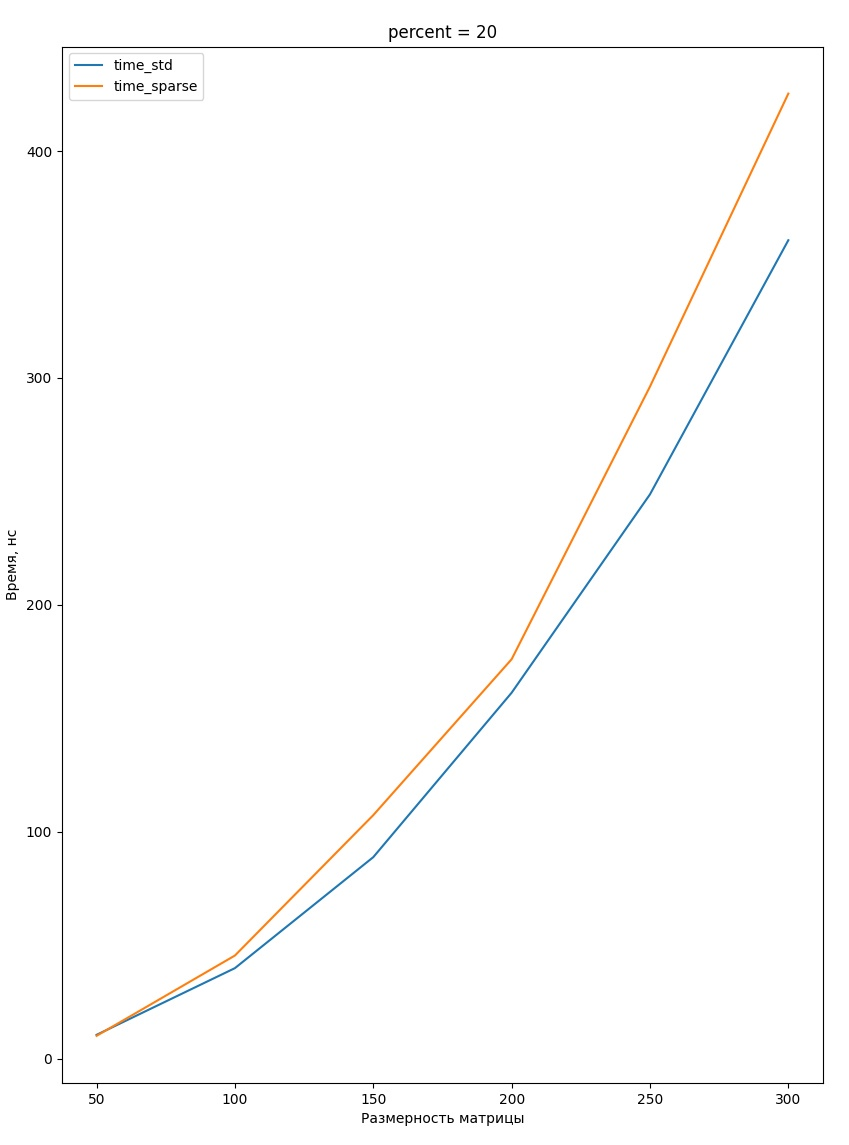
\includegraphics[width=\linewidth]{img/graph20.jpg}
	\label{graph20}
\end{figure}

\pagebreak

\begin{figure}
	\centering
	\caption{График зависимости времени от размерности матрицы при разреженности 80\%}
	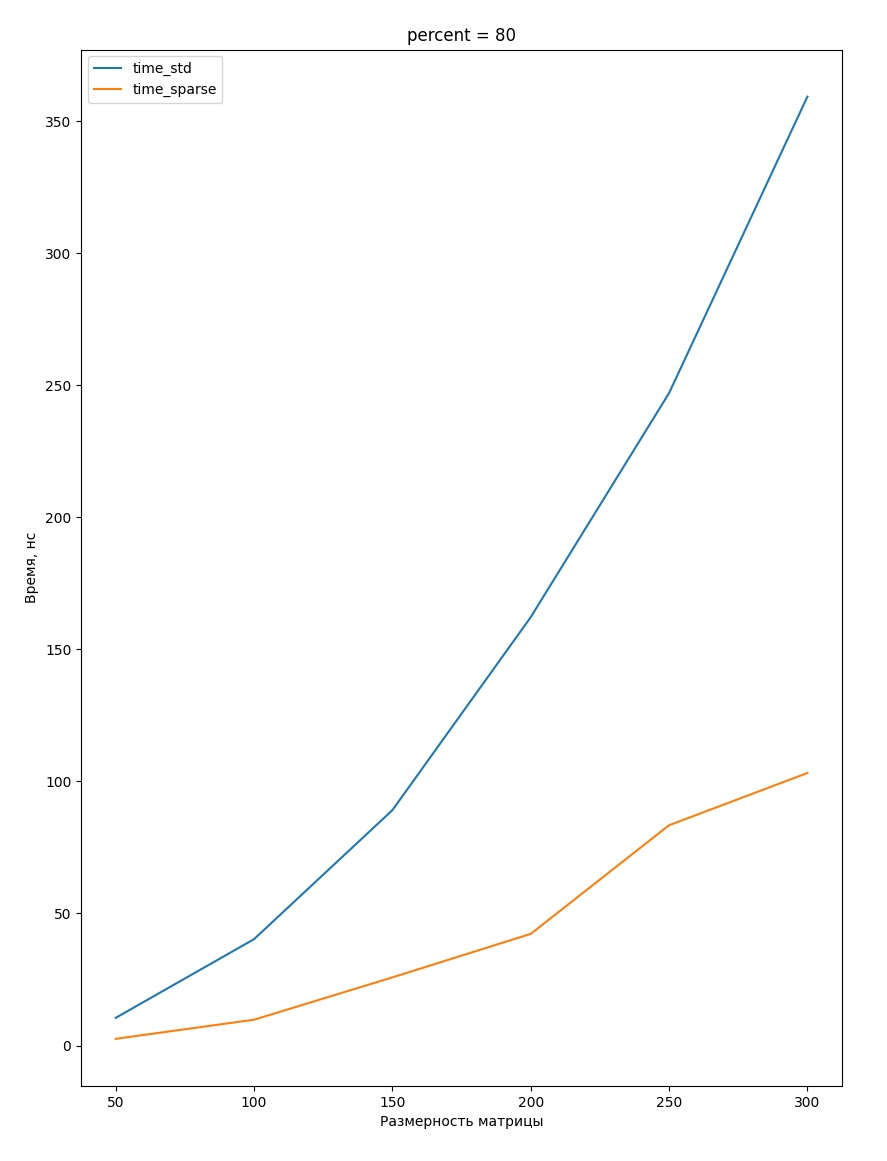
\includegraphics[width=\linewidth]{img/graph80.jpg}
	\label{graph80}
\end{figure}

\begin{figure}
	\centering
	\caption{График зависимости занимаемой матрицей памяти от процента заполненности ($100\times100$)}
	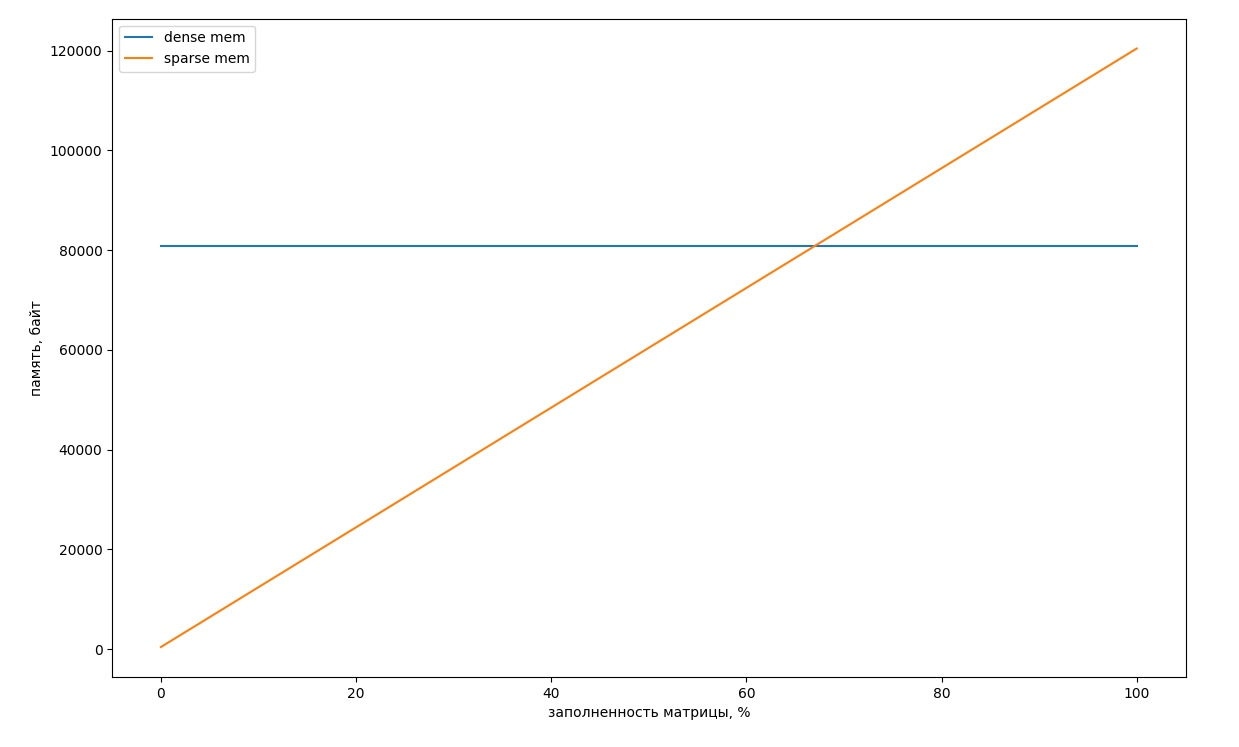
\includegraphics[width=0.8\linewidth]{img/mem.jpg}
	\label{mem}
\end{figure}

\begin{figure}
	\centering
	\caption{График зависимости занимаемой матрицей памяти от процента заполненности ($10\times10$)}
	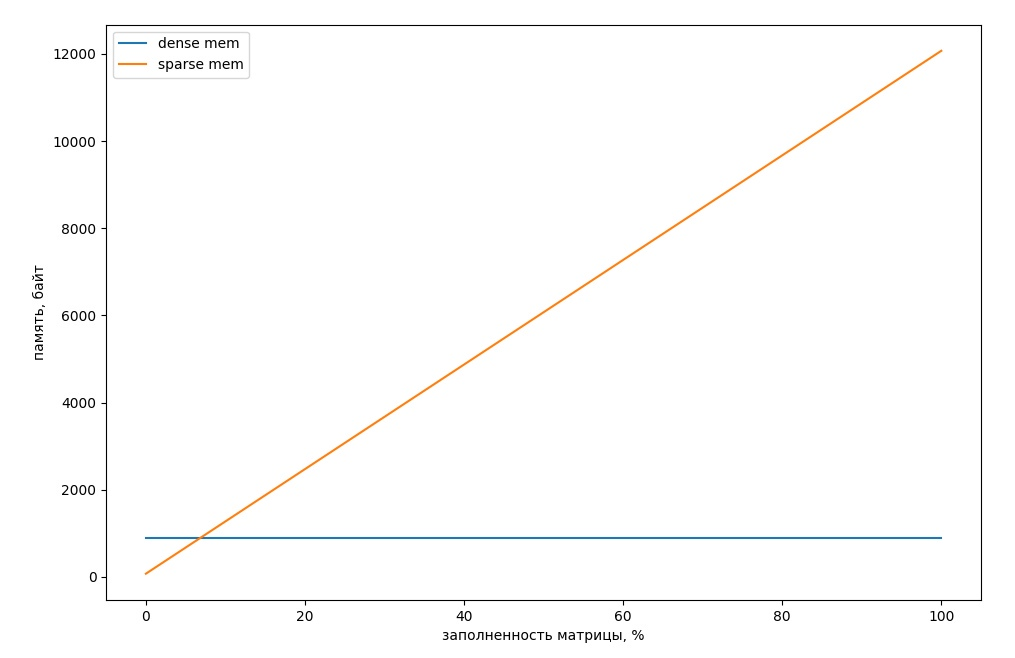
\includegraphics[width=0.8\linewidth]{img/mem10.jpg}
	\label{mem10}
\end{figure}

\pagebreak

\chapter{Контрольные вопросы}

\begin{enumerate}
	\item Что такое разреженная матрица, какие схемы хранения таких матриц Вы знаете?
	
	Разреженная матрица это структура данных, в которой хранятся только ненулевые элементы матрицы, и информация об их позиции в матрице. Такой информацией может быть, например явное указание строки и столбца (координатная форма), а может быть только индекс строки, но вместе с ненулевыми  элементами  тогда  хранится  список  индексов  элементов  с которых начинается тот или иной столбец в матрице (Йельский формат). Также,  в  ряде  случаев  работа  происходит  только  с  симетричными матрицами.  Тогда  нам  достаточно  хранить  только  половину  от  всех ненулевых элементов матрицы. Существует и множество других форматов, которые разрабатывались для определённой конфигурации матриц, и подходящие для очень узкого круга задач, например, можно хранить матрицу блоками.
	
	\item Каким  образом  и  сколько  памяти  выделяется  под  хранение разреженной и обычной матрицы? 
	
	Для хранения матрицы в обычном представлении память выделяется сразу под все элементы матрицы. Для  хранения  разреженной  матрицы  память  выделяется  по  мере необходимости и только для ненулевых элементов матрицы. При  этом,  для  хранения одного  элемента  в  разреженном  формате требуется  больше  памяти,  чем  в  обычном.  Тем  не  менее,  при  малой заполненности матрицы хранение только ненулевых элементов становится выгоднее.
	
	\item Каков принцип обработки разреженной матрицы?
	
	Принцип обработки разреженной матрицы заключается в том, чтобы обходить только ненулевые элементы матрицы, а не все возможные, тем самым облегчая сложность алгоритма с $O(N^2)$  до $O(K)$  где $N$  -  размерность матрицы, а $K$ - число ненулевых элементов в ней.
	
	\item В  каком  случае  для  матриц  эффективнее  применять стандартные алгоритмы обработки матриц? От чего это зависит? 
	
	Это зависит от выбранного формата хранения разреженной матрицы, а также в неменьшей степени от процента заполненности матрицы. Чем он меньше (разреженность выше), тем эффективнее использование алгоритмов, работающих с разреженными матрицами. Однако, если процент разреженности матрицы не превосходит $30-40\%$ то стандартные  алгоритмы  обработки  оказываются  не  только  проще,  но  и эффективнее нестандартных. 
\end{enumerate}


















